\documentclass[11pt, twoside, pdftex]{article}

% This includes all the settings that we should use for the document
\newcommand{\PDFTitle}{Bootable Embedded Systems for the DE0-Nano Board}
\newcommand{\commonPath}{../../Common}
\newcommand{\datePublished}{Mar 2022}

\newcommand{\versnum}{21.1} %version number quartus/AMP
\newcommand{\quartusname}{Quartus\textsuperscript{\textregistered} Prime}	
\newcommand{\textBar}{For \quartusname{} \versnum{}}
\newcommand{\thisyear}{2022 } %for copyright
\newcommand{\company}{FPGAcademy.org}
\newcommand{\longteamname}{FPGAcademy.org}
\newcommand{\teamname}{FPGAcademy}
\newcommand{\website}{FPGAcademy.org}

\newcommand{\productAcronym}{AMP}
\newcommand{\productNameShort}{Monitor Program}

\newcommand{\productNameMedTM}{Monitor Program}
\newcommand{\productNameMed}{Monitor Program}

%\newcommand{\headerLogoFilePath}[1]{#1/FPGAcademy.png}



\setlength\topmargin{-0.25in}
\setlength\headheight{0in}
\setlength\headsep{0.35in}
\setlength\textheight{8.5in}
\setlength\textwidth{7in}
\setlength\oddsidemargin{-0.25in}
\setlength\evensidemargin{-0.25in}
\setlength\parindent{0.25in}
\setlength\parskip{0in} 

\pdfpagewidth 8.5in
\pdfpageheight 11in

% listings is a package that supports encapsulating source code in LaTeX conveniently

\usepackage{listings}
% add support for graphics
\usepackage{graphicx}
\usepackage[usenames, dvipsnames]{color}

\def\expandparam\lstinputlisting[#1]#2{\edef\tmp{\noexpand\lstinputlisting[#1]{#2}}\tmp}

\widowpenalty 10000
\clubpenalty 10000

%%%%%%%%%%%%%%%%%%%% Source Code Formatting %%%%%%%%%%%%%%%%%%%%
\definecolor{globalCommentColour}{rgb}{0.588,0.588,0.588}

%%%%%%%%%%%%%%%%%%%%%%%%%%%%%%%%%%%%%%%%%%%%%%%%%%%%
% Defining a NiosII ASM highlighter for lstlisting
\lstdefinelanguage[NiosII]{Assembler} {
 	morekeywords={add, addi, and, andhi, andi, beq, bge, bgeu, bgt, bgtu, ble,  bleu, blt, bltu, bne, br, break,% 
 	bret, call, callr, cmpeq, cmpeqi, cmpge, cmpgei, cmpgeu, cmpgeui, cmpgt, cmpgti, cmpgtu, cmpgtui, cmple,%
 	cmplei, cmpleu, cmpleui, cmplt, cmplti, cmpltu, cmpltui, cmpne, cmpnei, custom, div, divu, eret, flushd,%
 	flushda, flushi, flushp, initd, initda, initi, jmp, jmpi, ldb, ldbio, ldbu, ldbuio, ldh, ldhio, ldhu, ldhuio,%
 	ldw, ldwio, mov, movhi, movi, movia, movui, mul, muli, mulxss, mulxsu, mulxuu, nextpc, nop, nor, or, orhi, ori,%
 	rdctl, rdprs, ret, rol, roli, ror, sll, slli, sra, srai, srl, srli, stb, stbio, sth, sthio, stw, stwio,%
 	sub, subi, sync, trap, wrctl, wrtcl, wrprs, xor, xori, xorhi, xori},% 	
 	morekeywords=[2]{.abort, .ABORT, .align, .app-file, .ascii, .asciz, .balign, .byte, .comm, .data, .def,%
 	.desc, .dim, .double, .eject, .else, .end, .endef, .endif, .equ, .equiv, .err, .extern, .file, .fill, .float,%
 	.global, .globl, .hword, .ident, .if, .include, .int, .irp, .irpc, .lcomm, .lflags, .line, .linkonce, .ln,%
 	.list, .long, .macro, .mri, .nolist, .octa, .org, .p2align, .psize, .quad, .rept, .sbttl, .scl, .section,%
 	.set, .short, .single, .size, .sleb128, .skip, .space, .stadb, .stabn, .stabs, .string, .symver, .tag,%
 	.text, .title, .type, .val, .uleb128, .word},% 	
 	morekeywords=[3]{et, bt, gp, sp, fp, ea, sstatus, ra, pc, status, estatus, bstatus, ienable, ipending, cpuid,%
 	exception, pteaddr, tlbacc, tlbmisc, eccinj, badaddr, config, mpubase, mpuacc},% 	
 	sensitive=t,%
 	alsoletter=.,%
	morestring=[b]",%
 	morecomment=[s]{/*}{*/},%
 	morecomment=[l]\#,%
   }[keywords,comments,strings]
   
   %% NOTE: morekeywords=[2] are GNU directives.
   
   \definecolor{niosInstructionColour}{rgb}{0.000,0.608,0.000}
   \definecolor{niosDirectiveColour}{rgb}{0.000,0.000,0.902}
   \definecolor{niosSpecialRegColour}{rgb}{0.000,0.000,0.000}
   \definecolor{niosStringColour}{rgb}{0.808,0.482,0.000}
   
   %% NOTE: To make bold use: =\bfseries\color{<colour>}
   \lstdefinestyle{defaultNiosStyle} {
   language=[NiosII]{Assembler},
   stringstyle=\color{niosStringColour},
   keywordstyle=\color{niosInstructionColour},
   keywordstyle=[2]\color{niosDirectiveColour},
   keywordstyle=[3]\itshape\color{niosSpecialRegColour}
   }
%%%%%%%%%%%%%%%%%%%%%%%%%%%%%%%%%%%%%%%%%%%%%%%%%%%%

%%%%%%%%%%%%%%%%%%%%%%%%%%%%%%%%%%%%%%%%%%%%%%%%%%%%
% Defining a ArmA9 ASM highlighter for lstlisting
\lstdefinelanguage[ArmA9]{Assembler} {
 	morekeywords={ADC, ADD, ADDS, AND, ANDS, B, BAL, BEQ, BGE, BGT, BL, BLT, BIC, BKPT, BLX, BNE, BX, CDP, CLZ, CMN, CMP, EOR,%
 	EORS, LDC, LDM, LDR, LDRB, LDRBT, LDRH, LDRSB, LDRSH, LDRT, LSL, MCR, MLA, MOV, MOVW, MOVT, MRC, MRS, MSR, MUL, MVN, ORR, PLD,%
 	ROR, RSB, RSC, SBC, SMLAL, SMULL, STC, STM, STR, STRB, STRBT, STRH, STRT, SUB, SUBS, SWI, SWP, SWPB, TEQ, UMLAL,
 	PUSH, POP, MOVS, RORS, LSR},%
 	morekeywords=[2]{.abort, .ABORT, .align, .app-file, .ascii, .asciz, .balign, .byte, .comm, .data, .def,%
 	.desc, .dim, .double, .eject, .else, .end, .endef, .endif, .equ, .equiv, .err, .extern, .file, .fill, .float,%
 	.global, .globl, .hword, .ident, .if, .include, .int, .irp, .irpc, .lcomm, .lflags, .line, .linkonce, .ln,%
 	.list, .long, .macro, .mri, .nolist, .octa, .org, .p2align, .psize, .quad, .rept, .sbttl, .scl, .section,%
 	.set, .short, .single, .size, .sleb128, .skip, .space, .stadb, .stabn, .stabs, .string, .symver, .tag,%
 	.text, .title, .type, .val, .vectors, .uleb128, .word},%
 	morekeywords=[3]{SP, PC, MIDR, CTR, TCMTR, TLBTR, MPIDR, ID_PFR0, ID_PFR1, ID_DFR0, ID_MMFR0, ID_MMFR1, ID_MMFR2,%
 	ID_MMFR3, ID_ISAR0, ID_ISAR1, ID_ISAR2, ID_ISAR3, ID_ISAR4, CCSIDR, CLIDR, AIDR, CSSELR, TTBR0, TTRB1, TTBR2, DACR,%
 	DFSR, IFSR, ADFSR, AIFSR, DFAAR, IFAR, ICIALLUIS, BPIALLIS, PAR, ICIALLU, ICIMVAU, BPIALL, DCIMVAC, DCISW, V2PCWPR,%
 	DCCVAC, DCCSW, DDIMVAC, DCISW, TLBALLIS, TLBIMVAIS, TLBIASIDIS, TLBIMVAAIS, TLBIALL, TLBIMVA, TLBIASID, TLBIMVAA,%
 	PMCR, PMCNTENSET, PMCNTENCLR, PMOVSR, PMSWINC, PMSELR, PMXEVTYPER, PMXEVCNTR, PMUSERENR, PMINTENSET, PMINTENCLR,%
 	PRRR, NRRR, PLEIDR, PLEASR, PLEFSR, PLEUAR, PLEPCR, VBAR, MVBAR, ISR, FCSEIDR, CONTEXTIDR, TPIDRURW, TPIDRURO, TPIDRPRW},%
 	sensitive=f,%
 	alsoletter=.,%
	morestring=[b]",%
 	morecomment=[s]{/*}{*/},%
 	morecomment=[l]{//},%
   }[keywords,comments,strings]
   
   %% NOTE: morekeywords=[2] are GNU directives.
   
   \definecolor{armInstructionColour}{rgb}{0.000,0.608,0.000}
   \definecolor{armDirectiveColour}{rgb}{0.000,0.000,0.902}
   \definecolor{armSpecialRegColour}{rgb}{0.000,0.000,0.000}
   \definecolor{armStringColour}{rgb}{0.808,0.482,0.000}
   
   \lstdefinestyle{defaultArmStyle} {
   language=[ArmA9]{Assembler},
   stringstyle=\color{armStringColour},
   keywordstyle=\color{armInstructionColour},
   keywordstyle=[2]\color{armDirectiveColour},
   keywordstyle=[3]\itshape\color{armSpecialRegColour}
   }
%%%%%%%%%%%%%%%%%%%%%%%%%%%%%%%%%%%%%%%%%%%%%%%%%%%%

%%%%%%%%%%%%%%%%%%%%%%%%%%%%%%%%%%%%%%%%%%%%%%%%%%%%
% Defining style for the verilog.

\definecolor{verilogCommentColour}{rgb}{0.000,0.502,0.000}

\lstdefinestyle{defaultVerilogStyle} {
language={Verilog},
keywordstyle=\color{blue},
commentstyle=\color{verilogCommentColour}
}
%%%%%%%%%%%%%%%%%%%%%%%%%%%%%%%%%%%%%%%%%%%%%%%%%%%%

%%%%%%%%%%%%%%%%%%%%%%%%%%%%%%%%%%%%%%%%%%%%%%%%%%%%
% Defining style for the vhdl.
\lstdefinestyle{defaultVHDLStyle} {
language={VHDL},
keywordstyle=\color{blue},
commentstyle=\color{verilogCommentColour}
}
%%%%%%%%%%%%%%%%%%%%%%%%%%%%%%%%%%%%%%%%%%%%%%%%%%%%

%%%%%%%%%%%%%%%%%%%%%%%%%%%%%%%%%%%%%%%%%%%%%%%%%%%%
% Java
\definecolor{javaStringColour}{rgb}{0.808,0.482,0}
%%%%%%%%%%%%%%%%%%%%%%%%%%%%%%%%%%%%%%%%%%%%%%%%%%%%

%%%%%%%%%%%%%%%%%%%%%%%%%%%%%%%%%%%%%%%%%%%%%%%%%%%%
% Defining language styles
% C
\definecolor{CStringColour}{rgb}{0.808,0.482,0}
%%%%%%%%%%%%%%%%%%%%%%%%%%%%%%%%%%%%%%%%%%%%%%%%%%%%

%%%%%%%%%%%%%%%%%%%%%%%%%%%%%%%%%%%%%%%%%%%%%%%%%%%%
% Defining extended LaTeX language.
\lstdefinelanguage[LocalLaTeX]{TeX}[LaTeX]{TeX}%
 	{moretexcs={bf, it, sf, lstset},%
   	}%

\lstdefinestyle{defaultLocalLatexStyle} {
language=[LocalLatex]{TeX},
keywordstyle=\color{blue}\bfseries,
keywordstyle=[2]\color{blue},
keywordstyle=[3]\color{blue}\bfseries
}
%%%%%%%%%%%%%%%%%%%%%%%%%%%%%%%%%%%%%%%%%%%%%%%%%%%%

\lstset{
%language = C,
%language = Verilog,
%basicstyle=\color{black}\rmfamily\ttfamily,
basicstyle=\small\color{black}\ttfamily,
commentstyle=\small\color{globalCommentColour}\itshape\ttfamily,
keywordstyle=\small\color{blue}\bfseries\ttfamily,
showstringspaces=false,
frame=none, %lines % boxed listings
breaklines=true,
breakatwhitespace=true,
tabsize=4
}
%%%%%%%%%%%%%%%%%%%%%%%%%%%%%%%%%%%%%%%%%%%%%%%%%%%%%%%%%%%%%%%%


%\usepackage[centering]{geometry}.
%%%%%%%%%%%%%%%%%%%%%%%%%%%%%%%%%%%%%%%%%%%%%%%%%%%
% Document Settings
\usepackage[labelsep=period]{caption}
% we can choose a better font later
%\usepackage{palatino}
\usepackage{fourier}
%\fontencoding{T1}
% include common used symbols
\usepackage{textcomp}
% add support for graphics
\usepackage{graphicx}
\usepackage[usenames, dvipsnames]{color}
% enable to draw thick or thin table hlines
\setlength{\doublerulesep}{\arrayrulewidth}
\usepackage{longtable}
\setlongtables
%\usepackage{array}
% It may be better to use PDFLaTeX as it can generate bookmarks for the
% document

% Add some useful packages
\usepackage{ae,aecompl}
\usepackage{epsfig,float,times}

% reset the font for section
\usepackage{sectsty}
%\allsectionsfont{\fontfamily{ptm}\selectfont}
\allsectionsfont{\usefont{OT1}{phv}{bc}{n}\selectfont}

% use compact space for sections
\usepackage[compact]{titlesec}
\titlespacing{\section}{0pt}{0.2in}{*0}
\titlespacing{\subsection}{0pt}{0.1in}{*0}
\titlespacing{\subsubsection}{0pt}{0.05in}{*0}

% fancyhdr header and footer customization
\usepackage{layout}
\usepackage{fancyhdr}
\pagestyle{fancy}
\fancyhead{}
\fancyhead[R]{\textit{\tiny{\textBar}}}
\fancyfoot{}
\fancyfoot[LO,
RE]{\textrm{\href{https://www.fpgacademy.org}{\small \longteamname}} \\ {\small \datePublished }}
\fancyfoot[RO, LE]{\small \thepage}
% two-side settings
%\fancyhead{} % clear all header fields
%\fancyfoot{} % clear all footer fields
%\fancyfoot[LE,RO]{\thepage}
\renewcommand{\headrulewidth}{2pt}
\renewcommand{\headrule}{{\color{blue} \hrule width\headwidth height\headrulewidth \vskip-\headrulewidth}}
\renewcommand{\footrulewidth}{0pt}

% Format the footer on page 1
\fancypagestyle{plain}{
\fancyhead{}
\fancyfoot{}
\fancyfoot[LO,
RE]{\textrm{\href{https://www.fpgacademy.org}{\small \longteamname}} \\ {\small \datePublished }}
\fancyfoot[RO, LE]{\small \thepage}
\renewcommand{\headrulewidth}{0pt}
}
% adjust some setting to try to make the figure stay in the same page with text
% Reference: 	http://www.cs.uu.nl/~piet/floats/node1.html
%   			http://mintaka.sdsu.edu/GF/bibliog/latex/floats.html
%   General parameters, for ALL pages:
\renewcommand{\topfraction}{0.9}	% max fraction of floats at top
\renewcommand{\bottomfraction}{0.8}	% max fraction of floats at bottom
%   Parameters for TEXT pages (not float pages):
\setcounter{topnumber}{3}
\setcounter{bottomnumber}{3}
\setcounter{totalnumber}{5}     % 2 may work better
\setcounter{dbltopnumber}{2}    % for 2-column pages
\renewcommand{\dbltopfraction}{0.9}	% fit big float above 2-col. text
\renewcommand{\textfraction}{0.07}	% allow minimal text w. figs
%   Parameters for FLOAT pages (not text pages):
\renewcommand{\floatpagefraction}{0.7}	% require fuller float pages
% N.B.: floatpagefraction MUST be less than topfraction !!
\renewcommand{\dblfloatpagefraction}{0.7}	% require fuller float pages
%%%%%%%%%%%%%%%%%%%%%%%%%%%%%%%%%%%%%%%%%%%%%%%%%%%
% remember to use [htp] or [htpb] for placement
%%%%%%%%%%%%%%%%%%%%%%%%%%%%%%%%%%%%%%%%%%%%%%%%%%%

% set no indent for paragraph
\setlength{\parindent}{0em}
\addtolength{\parskip}{11pt}
\newcommand{\compact}{[topsep=0pt]}
% use this package to reduce space
\usepackage{enumitem}
\usepackage{multirow}
\usepackage{rotating}
\usepackage{pifont}
\usepackage{dingbat}
\newcommand{\itemsecond}{$\circ$}
%
%%%%%%%%%%%%%%%%%%
\date{}
\author{}
%%%%%%%%%%%%%%%%%%
\newcommand{\de}{DE-series}
\newcommand{\up}{FPGAcademy}
\newcommand{\fabric}{Avalon Switch Fabric}
\newcommand{\TODO}[1]{\textcolor{red}{\textbf{TODO}: #1}}
\def\registered{{\ooalign{\hfil\raise .00ex\hbox{\scriptsize R}\hfil\crcr\mathhexbox20D}}}

% enable url and reference(bookmarks) in pdf
\usepackage{url}
\usepackage[pdftex, colorlinks]{hyperref}
\hypersetup{%
pdftitle={\PDFTitle},
linkcolor=blue,
hyperindex=true,
pdfauthor={\longteamname},
pdfkeywords={FPGAcademy, Academic Program, Example System},
bookmarksnumbered,
bookmarksopen=false,
filecolor=blue,
pdfstartview={FitH},
urlcolor=blue,
plainpages=false,
pdfpagelabels=true,
linkbordercolor={1 1 1} %no color for link border
}%
%%%%%%%%%%%%%%%%%%%%%%%%%%%%%%%%%%%%%%%%%%%%%%%%%%%
\setlength{\fboxsep}{0.7pt}
\setlength{\fboxrule}{0.5pt}

\newcommand{\red}[1]{{\color{red}\sf{#1}}}
\newcommand{\blue}[1]{{\color{blue}\sf{#1}}}



\usepackage{placeins}

%%%%%%%%%%%%%%%%%%%%%%%%%
% Add title
\newcommand{\doctitle}{Bootable Embedded Systems for the DE0-Nano Board}
\newcommand{\dochead}{Bootable Embedded Systems for the DE0-Nano Board}
% Usually no need to change these two lines
\title{\fontfamily{phv}\selectfont{\doctitle} }
\chead{ \small{\textsc{\bfseries \dochead} } }
% Customizations
%%%%%%%%%%%%%%%%%%%%%%%%%
% Allows multiple figures per page

\renewcommand\floatpagefraction{.9}
\renewcommand\topfraction{.9}
\renewcommand\bottomfraction{.9}
\renewcommand\textfraction{.1}   
\setcounter{totalnumber}{50}
\setcounter{topnumber}{50}
\setcounter{bottomnumber}{50}
\widowpenalty 10000
\clubpenalty 10000
\raggedbottom

%%%%%%%%%%%%%%%%%%
%%% DOCUMENT START
%\begin{document}
\begin{document}
\begin{table}
    \centering
    \begin{tabular}{p{5cm}p{4cm}}
        \hspace{-3cm}
        &
        \raisebox{1\height}{\parbox[h]{0.5\textwidth}{\Large\fontfamily{phv}\selectfont{\textsf{\doctitle}}}}
    \end{tabular}
    \label{tab:logo}
\end{table}

\colorbox[rgb]{0,0.384,0.816}{\parbox[h]{\textwidth}{\color{white}\textsf{\textit{\textBar}}}}

\thispagestyle{plain}

\section{Introduction}

This tutorial explains how the Intel\textsuperscript{\textregistered} DE0-Nano board can be configured such that, when
power is applied, it automatically loads an embedded system including the
Nios\textsuperscript{\textregistered} II processor and runs a boot program. Both the embedded system and Nios II boot program 
are stored in the non-volatile FPGA configuration device on the DE0-Nano board.
This tutorial assumes that the reader has a working knowledge of the C programming
language. It also assumes that the reader is familiar with the Intel
Quartus\textsuperscript{\textregistered} Prime and Platform Designer software, as well as the \productNameMed{}, and has access to a
computer on which this software is installed.

The screen shots in this tutorial were created using Quartus Prime version \versnum, Platform Designer,
and Monitor Program software. If other versions of the software are used, the screen
images may be slightly different.\\
\\
{\bf Contents:}

\begin{itemize}
\item Making a bootable embedded system for the DE0-Nano board
\item Writing a boot program for the Nios II processor, and storing this program in a 
memory initialization file
\item Changing the contents of the non-volatile FPGA configure device on the DE0-Nano board
\end{itemize}
\clearpage
\newpage

\section{Introduction}

A bootable embedded system for the DE0-Nano board can be created by following these steps:

\begin{enumerate}
\item Make an embedded system that includes a Nios II processor by using the Quartus Prime 
and Platform Designer software. Include an on-chip SRAM module in this embedded system. 

\item Set the address of the reset vector for the Nios II processor to be 
in the on-chip SRAM module.

\item Configure the on-chip SRAM module so that it will be initialized during FPGA programming.

\item Create the desired boot program that should be executed by the Nios II processor.  
Store the compiled boot program in a memory initialization file for the on-chip SRAM module.

\item Store the embedded system in the non-volatile FPGA configuration device on 
the DE0-Nano board.
\end{enumerate}

The above steps are described in detail in the following sections. 

\section{Making a Bootable Embedded System using Platform Designer}

For the purpose of this tutorial we will use the embedded system illustrated in
Figure \ref{fig:block_diagram}. This embedded system is called the {\it DE0-Nano Basic Computer},
and it is provided with the \productNameMed{} software. The source code for this system can
be found in the folder where the \productNameMed{} is installed on the reader's
computer: {\it$<$University\_Program\_Root\_Directory$>$ \textbackslash Computer\_Systems\textbackslash DE0-Nano\textbackslash DE0-Nano\_Basic\_Computer}. Note that a different embedded system can also be used with this tutorial, as
long as the system includes both a Nios~II processor and at least one on-chip SRAM module.

\begin{figure}[H]
   \begin{center}
        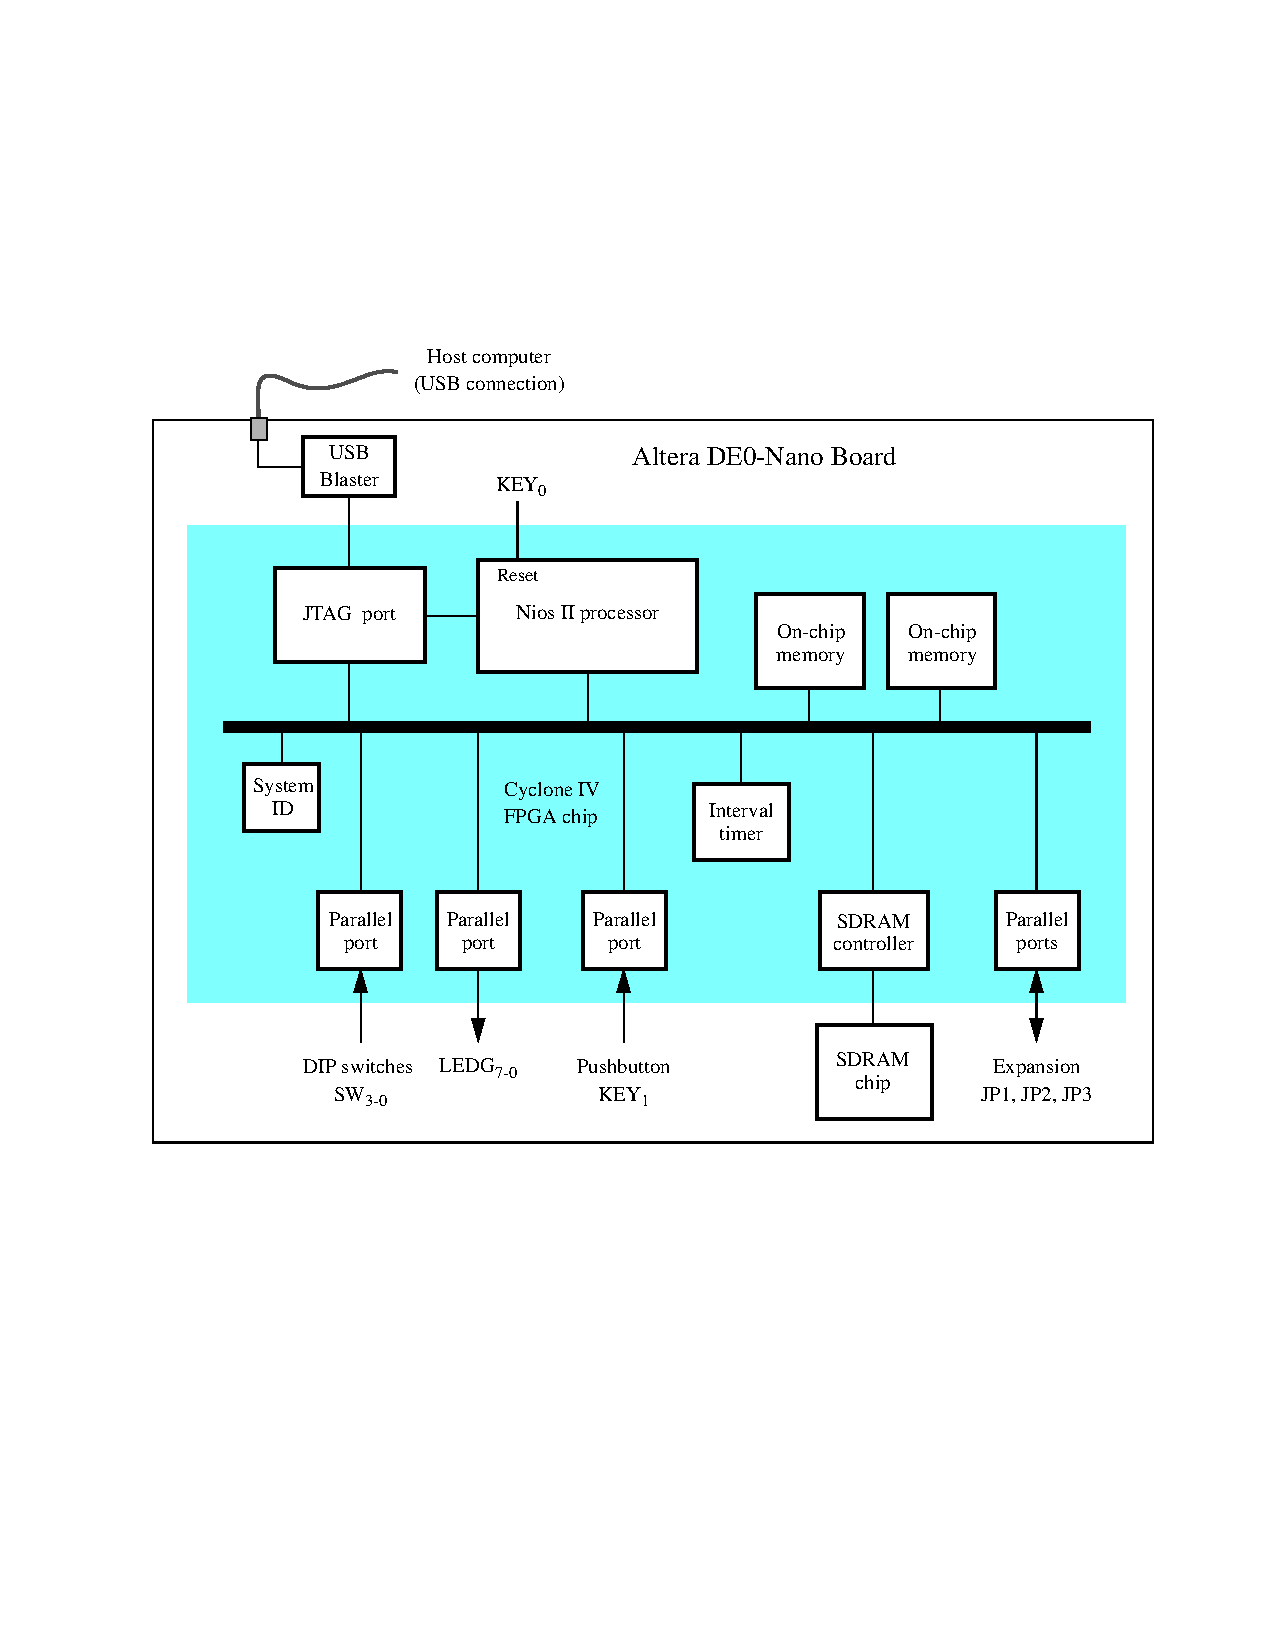
\includegraphics[width=0.99\textwidth]{figures/fig_block_diagram.pdf}
   \end{center}
   \caption{Block diagram of the DE0-Nano Basic Computer.}
	\label{fig:block_diagram}
\end{figure}

\newpage
\begin{figure}[H]
   \begin{center}
        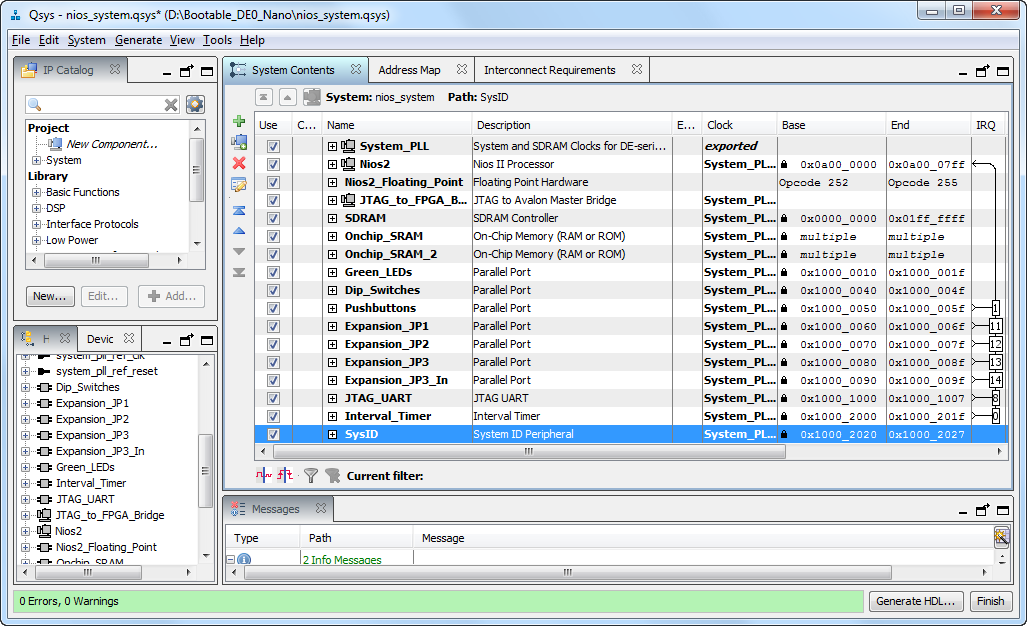
\includegraphics[width=0.99\textwidth]{figures/qsys.png}
   \end{center}
   \caption{The Platform Designer window for the DE0-Nano Basic Computer.}
	\label{fig:qsys}
\end{figure}

Create a copy of the source code of the DE0-Nano Basic Computer in a
folder named {\it Bootable\_DE0\_Nano}.  As mentioned earlier, this source code can
be found in the folder where the \productNameMed{} is installed.
In the DE0-Nano Basic Computer, the Nios II processor's 
reset vector is set to the starting address of the SDRAM module. To use the
DE0-Nano Basic Computer as a bootable system, the address of the Nios II reset vector 
has to be modified to use the on-chip SRAM module. To make this change, open the
Quartus Prime project for the DE0-Nano Basic Computer, which has the name 
{\it DE0\_Nano\_Basic\_Computer.qpf}. In the Quartus Prime software, open the Platform Designer
tool, as indicated in Figure \ref{fig:qsys}, and then open the settings for the Nios II 
processor, shown in Figure \ref{fig:reset_vector}.

\newpage
\begin{figure}[H]
   \begin{center}
        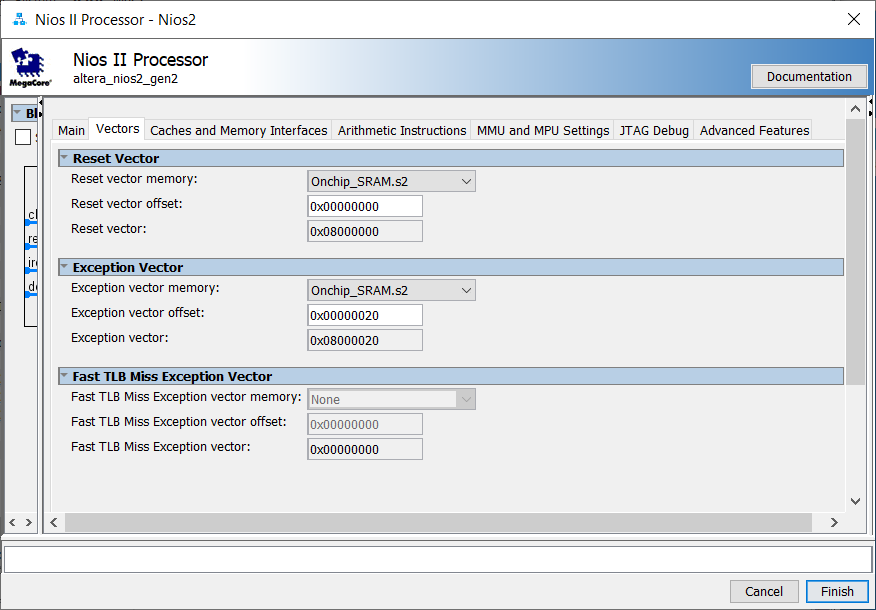
\includegraphics[width=0.8\textwidth]{figures/reset_vector.png}
   \end{center}
   \caption{Specifying the reset vector address.}
	\label{fig:reset_vector}
\end{figure}

Assign the {\sf Reset vector memory} for Nios II to
the module called {\it Onchip\_memory\_SRAM}, with an {\it offset} of 0. The address of
the reset vector is now set to the starting address of the on-chip SRAM module, 
which is {\sf 0x08000000}.

Figure \ref{fig:reset_vector} also shows that the Nios II exceptions vector is set to
the on-chip SRAM memory, at the address {\sf 0x08000020}.  This assignment is optional,
and does not have to use the same memory module as for the reset vector.

Since the Nios II processor will execute instructions in the on-chip SRAM module, the
contents of this memory have to be initialized during FPGA configuration. This is effected by
opening the settings windows for the on-chip SRAM module within Platform Designer, as illustrated in 
Figure \ref{fig:onchip_memory}. Under the {\sf Memory initialization} heading, 
select {\sf Initialize memory content}. Also, select {\sf Enable non-default
initialization file}, and specify the filename {\it boot\_code.hex}. This memory
initialization file will be created later in this tutorial.
% and will have a .{\it hex} filename extension. 

\newpage
\begin{figure}[H]
   \begin{center}
        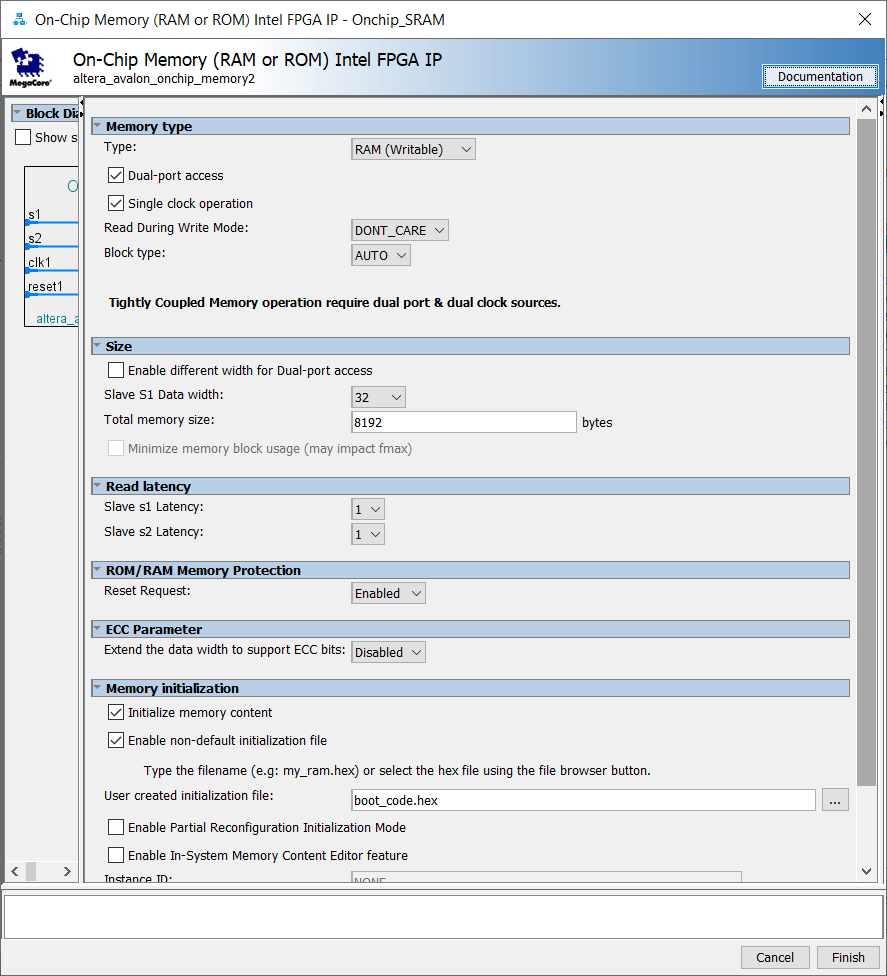
\includegraphics[width=0.6\textwidth]{figures/onchip_memory.png}
   \end{center}
   \caption{Specifying a memory initialization file.}
	\label{fig:onchip_memory}
\end{figure}

After the Nios II processor and on-chip SRAM module have been configured as needed,
a new embedded system can be generated by using Platform Designer. Open the {\sf Generation} window by selecting {\sf Generate > Generate HDL ...} in 
the Platform Designer window and then click on the {\sf Generate} button. 
After the embedded system has been successfully generated, the Platform Designer tool can be closed.
Now, in Quartus~Prime recompile the DE0-Nano Basic Computer project to produce a new FPGA 
programming file, which is called {\it DE0\_Nano\_Basic\_Computer.sof}. We should note
that we have not yet created the memory initialization file that 
was specified in Figure \ref{fig:onchip_memory}. Quartus Prime allows the project to be 
compiled without including this file---we will create the memory initialization file,
called {\it boot\_code.hex}, later in this tutorial, and then compile the Quartus 
Prime project again.

\section{Creating a Boot Program for the Nios\textsuperscript{\textregistered} II Processor}

A boot program provides the code that the Nios II processor executes when power is
applied, or a reset is performed. For this tutorial we use a small
example of a boot program that performs the simple task of scrolling a light back and
forth across the green LEDs on the DE0-Nano board. This program is provided only as an
example to illustrate the steps involved---in a real application a boot program would perform a
more useful task.  In many practical applications it may be desirable on power-up to 
run a Nios II program that is too large to fit into the provided on-chip SRAM module. In 
such cases, the boot program would be designed to load a larger program from a non-volatile
storage location, such as the EEPROM chip on the DE0-Nano board, into the SDRAM chip.

The example boot program for this tutorial is shown in Figure \ref{fig:boot_code}.
It uses memory mapped I/O to load a pattern into the parallel port of the DE0-Nano Basic
Computer that is connected to the green LEDs on the DE0-Nano board. The pattern is
repeatedly displayed on the LEDs after being shifted in the right or left direction. The
frequency of shifting and displaying the pattern is controlled by using the interval timer 
in the DE0-Nano Basic Computer. 

Type the code in Figure \ref{fig:boot_code} into a file with the name {\it boot\_code.c}.

\begin{figure}[!h]
\lstinputlisting[language=C]{design_files/boot_code.c}
\caption{The boot program.}
\label{fig:boot_code}
\end{figure}

\clearpage
\newpage

To compile and test the boot program, ensure that a DE0-Nano board is plugged into your
computer. Then, open the \productNameMed{} software. 
In the Monitor Program, create a new project by using the New Project Wizard.  Give the
project the name {\it boot\_code}. In the {\sf Select a system} 
screen of the New Project Wizard, choose {\sf Custom System}, as
illustrated in Figure \ref{fig:select_system}, and browse to select the embedded 
system called {\it nios\_system.qsys} that we created using the Platform Designer tool
in the {\it Bootable\_DE0\_Nano} folder. Also browse to select the {\sf Quartus Prime programming
(SOF) file} that we made in the previous step of this tutorial, 
named {\it DE0\_Nano\_Basic\_Computer.sof}. 

\begin{figure}[H]
   \begin{center}
        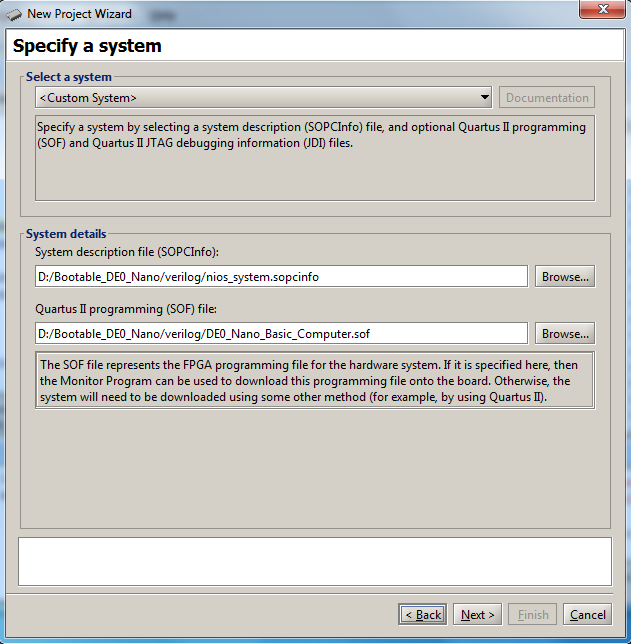
\includegraphics[scale=.65]{figures/select_system.png}
   \end{center}
   \caption{Selecting the bootable embedded system.}
	\label{fig:select_system}
\end{figure}

Click {\sf Next} in the New Project Wizard, and in the {\sf Specify a program type} screen 
select {\it C Program}.  Next, in the {\sf Specify program details} screen click 
the {\sf Add} button and choose the {\it boot\_code.c} file. Accept the default 
settings in the {\sf Specify system parameters} screen, including the specification of the
{\it USB-Blaster} cable that is connected to your DE0-Nano board. Finally, in the 
{\sf Specify program memory settings} screen, shown in Figure \ref{fig:text_data}, 
set the .{\it text} section of the Nios II program to the on-chip SRAM module. 

\begin{figure}[H]
   \begin{center}
        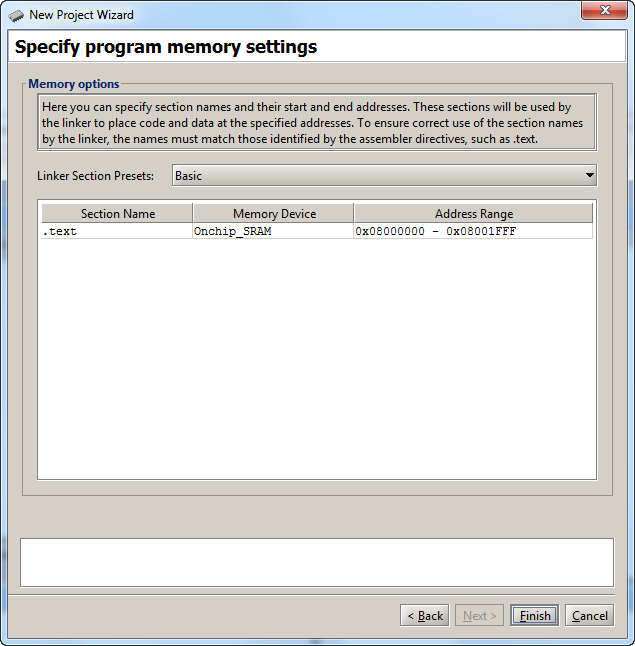
\includegraphics[scale=.8]{figures/text_data.png}
   \end{center}
   \caption{Specifying the memory module for the text and data sections.}
	\label{fig:text_data}
\end{figure}

Compile the {\it boot\_code} project in the Monitor Program and download it into your
DE0-Nano board. Run the program and observe the scrolling pattern on the green lights.

As a result of compiling the {\it boot\_code} project an executable file named
{\it boot\_code.elf} was created, and then downloaded into the on-chip SRAM module by the 
Monitor Program. To use this executable file as a boot program, we need to store it in the
memory initialization file that we specified in Figure \ref{fig:onchip_memory}, and then
include this file in the data that is stored in the non-volatile FPGA configuration device
on the DE0-Nano board. We need to first convert the {\it elf} file it into a different 
format, as described below. 

\subsection{Using a Memory Initialization File}

To make a memory initialization file, we need to convert the {\it boot\_code.elf} file
into a format known as {\it Intel HEX} format. To perform the conversion select the
Monitor Program command {\sf Actions} $>$ {\sf Convert Program to Hex File}. This command
will create a file in Intel HEX format with the name {\it nios\_system\_Onchip\_SRAM.hex}.
Rename the file {\it boot\_code.hex}.

Make sure that a copy of the {\it boot\_code.hex} file is present in the 
{\it Bootable\_DE0\_Nano} folder where the Quartus Prime project for this tutorial is stored.
Then, recompile the project in Quartus Prime to make a new FPGA programming file, which is named 
{\it DE0\_Nano\_Basic\_Computer.sof}.  Since we specified, in Figure \ref{fig:onchip_memory},
that {\it boot\_code.hex} should be used to initialize the on-chip SRAM module, then 
the {\it SOF} file produced by Quartus Prime will now contain this information. We can
permanently store the contents of this {\it SOF} file into the non-volatile
FPGA configuration device on the DE0-Nano board as described in the following section.

\section{Programming the Non-volatile FPGA Configuration Device}

To program the non-volatile FPGA configuration device on the DE0-Nano board we need to use
a method called {\it JTAG* Indirect Configuration}. To create the programming information
needed for this method, in the Quartus Prime software select the command {\sf File} $>$
{\sf Convert Programming Files}. In the window shown in Figure \ref{fig:jic1}, click 
on the pull-down menu next to {\sf Programming file type} and select {\sf JTAG Indirect Configuration File (.jic)}.

\begin{figure}[H]
   \begin{center}
        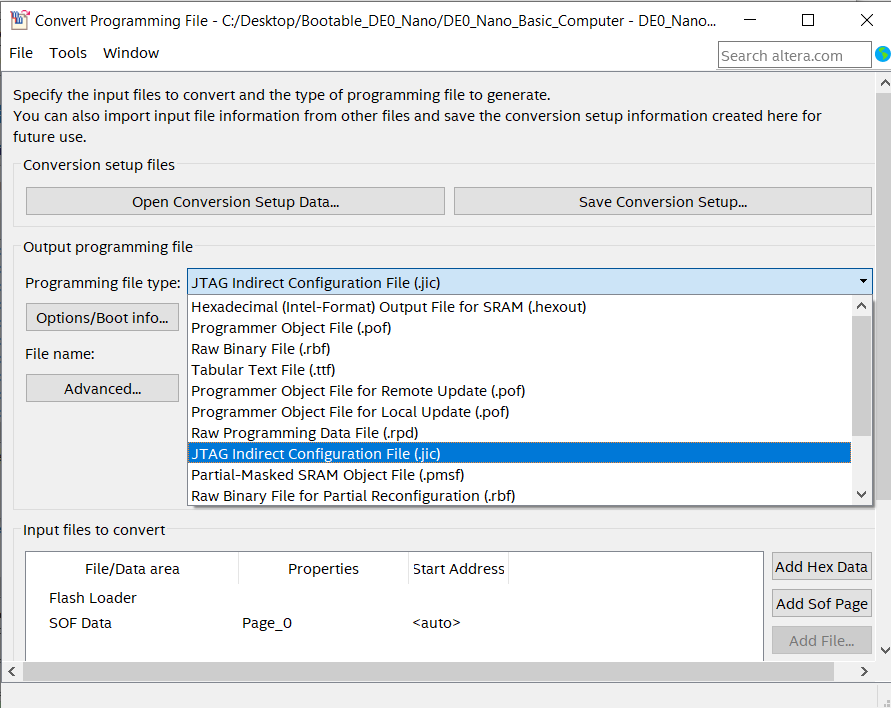
\includegraphics[scale=.5]{figures/jic1.png}
   \end{center}
   \caption{Choosing the programming file type.}
	\label{fig:jic1}
\end{figure}

As illustrated in Figure \ref{fig:jic2}, make the following settings. Under {\sf Configuration
device} select either {\it EPCS64} (for most DE0-Nano boards) or {\it EPCS16} (for older DE0-Nano
boards). In the {\sf File name} box specify a meaningful name for the file that will be
generated, such as {\it Bootable\_DE0\_Nano.jic}.  Next, as indicated in the figure, 
in the {\sf Input files to convert} area click to highlight the line {\sf SOF Data}, 
and and click {\sf Add File} to browse to select the file {\it DE0\_Nano\_Basic\_Computer.sof}.

\begin{figure}[H]
   \begin{center}
        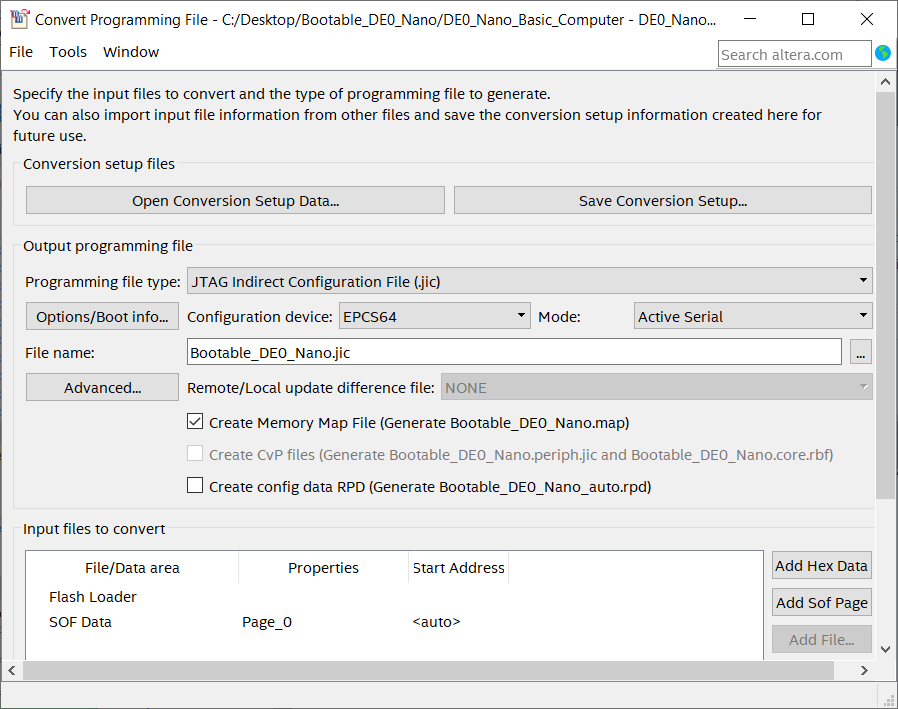
\includegraphics[scale=.5]{figures/jic2.png}
   \end{center}
   \caption{Additional settings.}
	\label{fig:jic2}
\end{figure}

Next, click to highlight 
the line {\sf Flash Loader} and then click {\sf Add Device}, as shown in Figure \ref{fig:jic3}.
Select the {\sf Cyclone\textsuperscript{\textregistered} IV E} device on the DE0-Nano board, which is called {\sf EP4CE22}, as
depicted Figure \ref{fig:jic4}. 

\begin{figure}[H]
   \begin{center}
        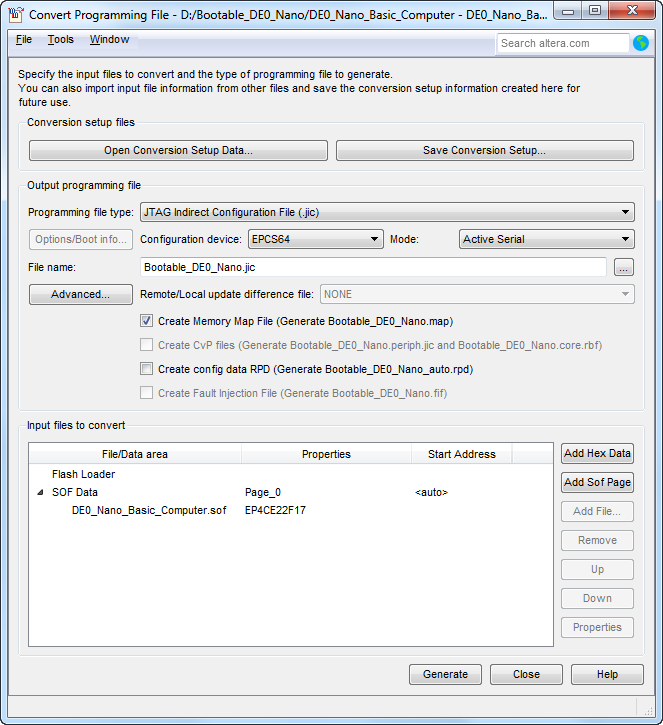
\includegraphics[scale=.5]{figures/jic3.png}
   \end{center}
   \caption{Adding the JTAG Indirect Configuration device.}
	\label{fig:jic3}
\end{figure}

\begin{figure}[H]
   \begin{center}
        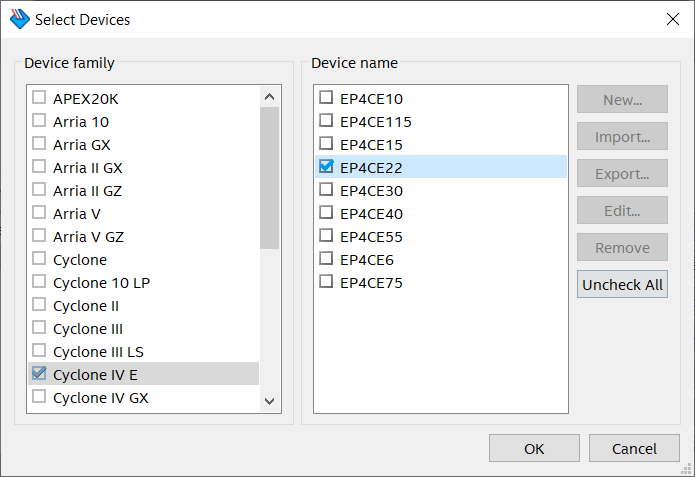
\includegraphics[scale=.5]{figures/jic4.png}
   \end{center}
   \caption{Choosing the EP4CE22 device.}
	\label{fig:jic4}
\end{figure}

Finally, under {\sf SOF Data} click to select the filename 
{\it DE0\_Nano\_Basic\_Computer.sof} that we added previously. Click {\sf Properties}
on the righthand side of the screen in Figure \ref{fig:jic3} to open the window in 
Figure \ref{fig:jic5}, and click to select {\sf Compression}.

\begin{figure}[H]
   \begin{center}
        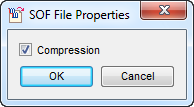
\includegraphics[scale=.6]{figures/jic5.png}
   \end{center}
   \caption{The Properties window.}
	\label{fig:jic5}
\end{figure}

To produce the {\it Bootable\_DE0\_Nano.jic} programming file, click the {\sf Generate} button
on the bottom of the screen in Figure \ref{fig:jic3}.

\subsection{Downloading the JIC file into the DE0-Nano Board}

To load the generated JIC file into the non-volatile FPGA configuration device on the DE0-Nano
board, open the Quartus Prime Programmer. Ensure that the \productNameMed{} software
is closed (or disconnected from the DE0-Nano board), because the Quartus Prime 
Programmer cannot communicate with the DE0-Nano board if it is already connected to 
the Monitor Program.

In the window shown in Figure \ref{fig:programmer} make sure that the 
USB-Blaster connected to your DE0-Nano
board is shown in the {\sf Hardware Setup} box. If any programming file, such as the 
{\it DE0\_Nano\_Basic\_Computer.sof}, is listed in the Programmer window, then click to
select this file and then click on the {\sf Delete} button. Next, click the {\bf Add File}
button and browse to choose the {\it Bootable\_DE0\_Nano.jic} file. Check the
{\sf Program/Configure}, {\sf Verify}, and {\sf Blank-Check} selections, as shown in the 
figure, and then click on the {\sf Start} button.

The Quartus Prime Programmer will download the JIC file into the non-volatile FPGA
configuration device. Once the programming task is completed, power-cycle the DE0-Nano
board and verify that it automatically loads and executes the boot program.

\begin{figure}[H]
   \begin{center}
        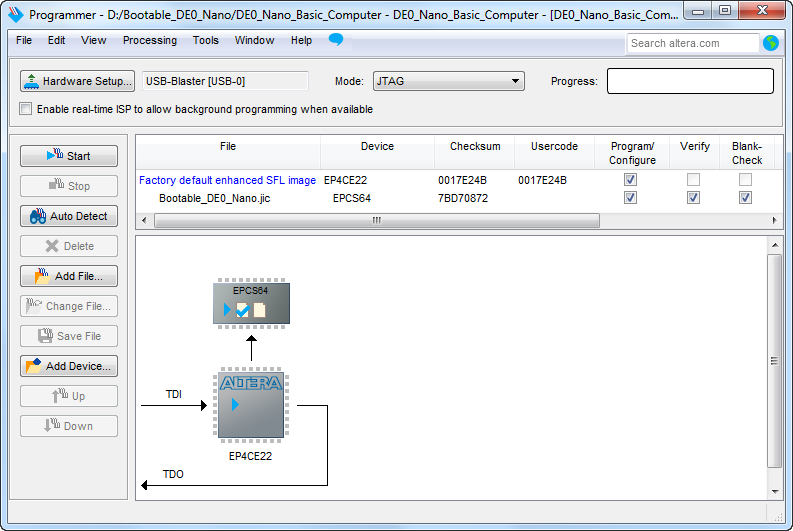
\includegraphics[scale=.5]{figures/programmer.png}
   \end{center}
   \caption{The Programmer window.}
	\label{fig:programmer}
\end{figure}

% Copyright and Trademark

%\newcommand{\datePublished}{Mar 2022}

\newcommand{\versnum}{21.1} %version number quartus/AMP
\newcommand{\quartusname}{Quartus\textsuperscript{\textregistered} Prime}	
\newcommand{\textBar}{For \quartusname{} \versnum{}}
\newcommand{\thisyear}{2022 } %for copyright
\newcommand{\company}{FPGAcademy.org}
\newcommand{\longteamname}{FPGAcademy.org}
\newcommand{\teamname}{FPGAcademy}
\newcommand{\website}{FPGAcademy.org}

\newcommand{\productAcronym}{AMP}
\newcommand{\productNameShort}{Monitor Program}

\newcommand{\productNameMedTM}{Monitor Program}
\newcommand{\productNameMed}{Monitor Program}

%\newcommand{\headerLogoFilePath}[1]{#1/FPGAcademy.png}



%%%%%%%%%%%%%%%%%%%%%%%%%%%%%%%%%%%%%%%%
%%% FPGAcademy Copyright Information %%%
%%%%%%%%%%%%%%%%%%%%%%%%%%%%%%%%%%%%%%%%

%Always put the copyright on a new page (clear page), with some vertical space from top
\clearpage
\vspace{1in}

\noindent

Copyright {\copyright} FPGAcademy.org. All rights reserved. FPGAcademy and the FPGAcademy logo are trademarks of  FPGAcademy.org.  This document is being provided on an ``as-is'' basis and as an accommodation and therefore all warranties, representations or guarantees of any kind (whether express, implied or statutory) including, without limitation, warranties of merchantability, non-infringement, or fitness for a particular purpose, are specifically disclaimed.

%FPGAcademy assumes no responsibility or liability arising out of the application or use of any information,  product,  or  service  described  herein  except  as  expressly  agreed  to  in  writing  by  FPGAcademy.



**Other names and brands may be claimed as the property of others.




\end{document}

